\documentclass[main]{subfiles}

\begin{document}

\chapter{Manual de usuario}
\label{chap:anexo_manual}

Este manual de usuario indica los pasos a seguir para volar el cuadric\'optero en modo hovering. Se asume que la IMU se encuentra previamente calibrada. 

\section{Montaje y conexionado}

\subsubsection{Componentes del sistema}
Montar sobre la plataforma los distintos componentes del sistema:
\begin{itemize}
\item BeagleBoard, BeagleJuice y m\'odulo de WiFi en la caja de acr\'ilico como se detalla en el cap\'itulo \ref{chap:montaje}.
\item IMU
\item ESC
\item GPS
\item Placa de conversi\'on de niveles l\'ogicos
\item Bater\'ia
\end{itemize}
Si se desea utilizar la opci\'on de utilizar el control remoto debe incluirse la CPU de f\'abrica, el receptor y el circuito encargado del switcheo (ver cap\'itulo \ref{chap:anexo_switcheo}).

\subsubsection{Conexiones}
En esta secci\'on se detallan las conexiones de los componentes.
\begin{itemize}
\item Conexiones de la BeagleBoard
	\begin{itemize}
	\item Conectar la BeagleBoard a la BeagleJuice
	\item Conectar en un puerto USB el módulo de WiFi, en otro el GPS y en un tercero un pendrive.
	\item Conexión con la placa de conversión de niveles lógicos. Sobre esta \'ultima se encuentran indicados los nombres de las señales. Referirse a la p\'agina 108 del BeagleBoard-xM System Reference Manual.
	\end{itemize}
\item Conexiones de la IMU
	\begin{itemize}
	\item Conectar la alimentaci\'on a la BeagleJuice
	\item Conectar las señales de Gnd, 3.3V, Tx y Rx a la placa de conversión de niveles l\'ogicos
	\end{itemize}
\item Conexión de los ESCs
	\begin{itemize}
	\item Conectar las lineas del I2C (SDA, SCLK, GND) a la placa de conversión de niveles l\'ogicos.
	\item Conectar a los motores. En la figura \ref{fig:conexion_motores} puede observarse la correspondencia entre ESC y motores.
	\item Conectar la bater\'ia
	\end{itemize}
\end{itemize}

En caso de desearse utilizar también el control remoto, conectar la CPU de f\'abrica y el circuito de Switcheo de acuerdo a las conexiones que se especif\'ican en el cap\'itulo \ref{chap:anexo_switcheo}.

\begin{figure}
	\centering
	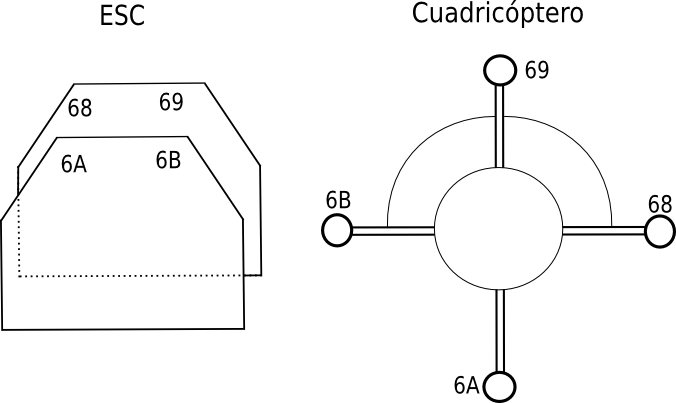
\includegraphics[width=0.7\textwidth]{./pics_manual/diagrama.png}
	\caption{Correspondencia entre motores y ESC}
	\label{fig:conexion_motores}
\end{figure}

Se debe hacer coincidir el plano de la IMU con el plano formado por los motores de acuerdo al procedimiento explicado en el cap\'iutlo \ref{chap:montaje}. Para imprimir en consola las medidas de la IMU en consola debe ejecutarse:
\begin{verbatim}
ssh root@10.42.43.2
cd work/uquad/src/build/test/imu_comm_test
./imu_comm_test /dev/ttyS1
\end{verbatim}

Las columnas 10 a 12 indican los \'angulos de Euler. Se deben ajustar los tornillos de la IMU hasta que dichos \'angulos sean lo m\'as cercano posible al cero.

\section{Ajuste del Offset}
\begin{itemize}
\item Offset del \'angulo de Yaw
	\begin{enumerate}
	\item Colgar el cuadric\'optero de forma que pueda girar respecto al eje vertical. 
	\item Correr ./cmdstdin a una velocidad de I2C lo m\'as alta posible sin que el cuadric\'optero se levante (Se sugiere utilizar 120 I2C). Dicho programa se encuentra en work/uquad/i2c\_beagle/ 
	\item Ajustar los offset de los motores en work/uquad/src/i2c\_beagle/cmd\_motores.c hasta que el cuadric\'optero no gire.
	\end{enumerate}
\item Offset del \'angulo de Pitch y de Roll
	\begin{enumerate}
	\item Ubicar el caudric\'optero de forma que tenga libre un solo eje de giro posible.
	\item Igual que en el caso anterior ajustar el offset de forma que el cuadric\'optero se mantenga horizontal.
	\item Repetir para el otro \'angulo
	\end{enumerate}	
\end{itemize}

\section{Pruebas del Controlador}
\begin{itemize}
\item Prueba de los \'angulos de Roll y de Pitch
	\begin{enumerate}
	\item Ubicar el caudric\'optero de forma que tenga libre un solo eje de giro posible. Modificar las matrices K\_prop\_full\_ppzt.txt y K\_int\_full\_ppzt.txt de forma que las unicas entradas distintas de cero sean las que corresponden a la realimentaci\'on del \'angulo de inter\'es, de la velocidad angular de inter\'es y de la integral del error del \'angulo de inter\'es. Las matrices de realimentaci\'on se encuentran en work/uquad/src/control.
	\item Correr el loop de control (./go.sh), modificar dichas matrices hasta encontrarse conforme con la respuesta del sistema.
	\item Repetir con el otro \'angulo
	\end{enumerate}
\item Prueba del \'angulo de Yaw
	\begin{enumerate}
	\item Colgar el cuadric\'optero
	\item Setear la Masa del cuadric\'optero lo m\'as alto posible sin que el cuadric\'optero levante vuelo (se sugiere utilizar 1.4Kg)
	\item Modificar las matrices K\_prop\_full\_ppzt.txt y K\_int\_full\_ppzt.txt hasta lograr el comportamiento deseado
	\end{enumerate}
\end{itemize}
Una vez realizadas las pruebas anteriores el cuadric\'optero deber\'ia presentar un comportamiento estable. De todas formas se sugiere agregar dos cuerdas de seguridad: una por encima y otra por debajo, de forma de limitar el movimiento del mismo y evitar accidentes. 
\end{document}